% -----------------------------------------------
% Template for ICMC SMC 2014
% adapted and corrected from the template for SMC 2013,  which was adapted from that of  SMC 2012, which was adapted from that of SMC 2011
% -----------------------------------------------

\documentclass{article}
\usepackage{icmcsmc2014}
\usepackage{times}
\usepackage{ifpdf}
\usepackage[english]{babel}
%\usepackage{cite}

%%%%%%%%%%%%%%%%%%%%%%%% Some useful packages %%%%%%%%%%%%%%%%%%%%%%%%%%%%%%%
%%%%%%%%%%%%%%%%%%%%%%%% See related documentation %%%%%%%%%%%%%%%%%%%%%%%%%%
%\usepackage{amsmath} % popular packages from Am. Math. Soc. Please use the 
%\usepackage{amssymb} % related math environments (split, subequation, cases,
%\usepackage{amsfonts}% multline, etc.)
%\usepackage{bm}      % Bold Math package, defines the command \bf{}
%\usepackage{paralist}% extended list environments
%%subfig.sty is the modern replacement for subfigure.sty. However, subfig.sty 
%%requires and automatically loads caption.sty which overrides class handling 
%%of captions. To prevent this problem, preload caption.sty with caption=false 
%\usepackage[caption=false]{caption}
%\usepackage[font=footnotesize]{subfig}


%user defined variables
\def\papertitle{}
\def\firstauthor{Spencer Salazar}
\def\secondauthor{Ge Wang}

% adds the automatic
% Saves a lot of ouptut space in PDF... after conversion with the distiller
% Delete if you cannot get PS fonts working on your system.

% pdf-tex settings: detect automatically if run by latex or pdflatex
\newif\ifpdf
\ifx\pdfoutput\relax
\else
   \ifcase\pdfoutput
      \pdffalse
   \else
      \pdftrue
\fi

\ifpdf % compiling with pdflatex
  \usepackage[pdftex,
    pdftitle={\papertitle},
    pdfauthor={\firstauthor, \secondauthor},
    bookmarksnumbered, % use section numbers with bookmarks
    pdfstartview=XYZ % start with zoom=100% instead of full screen; 
                     % especially useful if working with a big screen :-)
   ]{hyperref}
  %\pdfcompresslevel=9

  \usepackage[pdftex]{graphicx}
  % declare the path(s) where your graphic files are and their extensions so 
  %you won't have to specify these with every instance of \includegraphics
  \graphicspath{{./figures/}}
  \DeclareGraphicsExtensions{.pdf,.jpeg,.png}

  \usepackage[figure,table]{hypcap}

\else % compiling with latex
  \usepackage[dvips,
    bookmarksnumbered, % use section numbers with bookmarks
    pdfstartview=XYZ % start with zoom=100% instead of full screen
  ]{hyperref}  % hyperrefs are active in the pdf file after conversion

  \usepackage[dvips]{epsfig,graphicx}
  % declare the path(s) where your graphic files are and their extensions so 
  %you won't have to specify these with every instance of \includegraphics
  \graphicspath{{./figures/}}
  \DeclareGraphicsExtensions{.eps}

  \usepackage[figure,table]{hypcap}
\fi

%setup the hyperref package - make the links black without a surrounding frame
\hypersetup{
    colorlinks,%
    citecolor=black,%
    filecolor=black,%
    linkcolor=black,%
    urlcolor=black
}

\hyphenpenalty=50

% Title.
% ------
\title{miniAudicle for iPad \\ Touchscreen-based Music Software Programming}

%Two addresses
%--------------
 \twoauthors
   {\firstauthor} { %
     {\tt \href{mailto:spencer@ccrma.stanford.edu}{spencer@ccrma.stanford.edu}}}
   {\secondauthor} { %
     {\tt \href{mailto:ge@ccrma.stanford.edu}{ge@ccrma.stanford.edu}}}

\jointaffil{Center for Computer Research in Music and Acoustics (CCRMA) \\ Stanford University \\ Stanford, CA}

\teaser{
	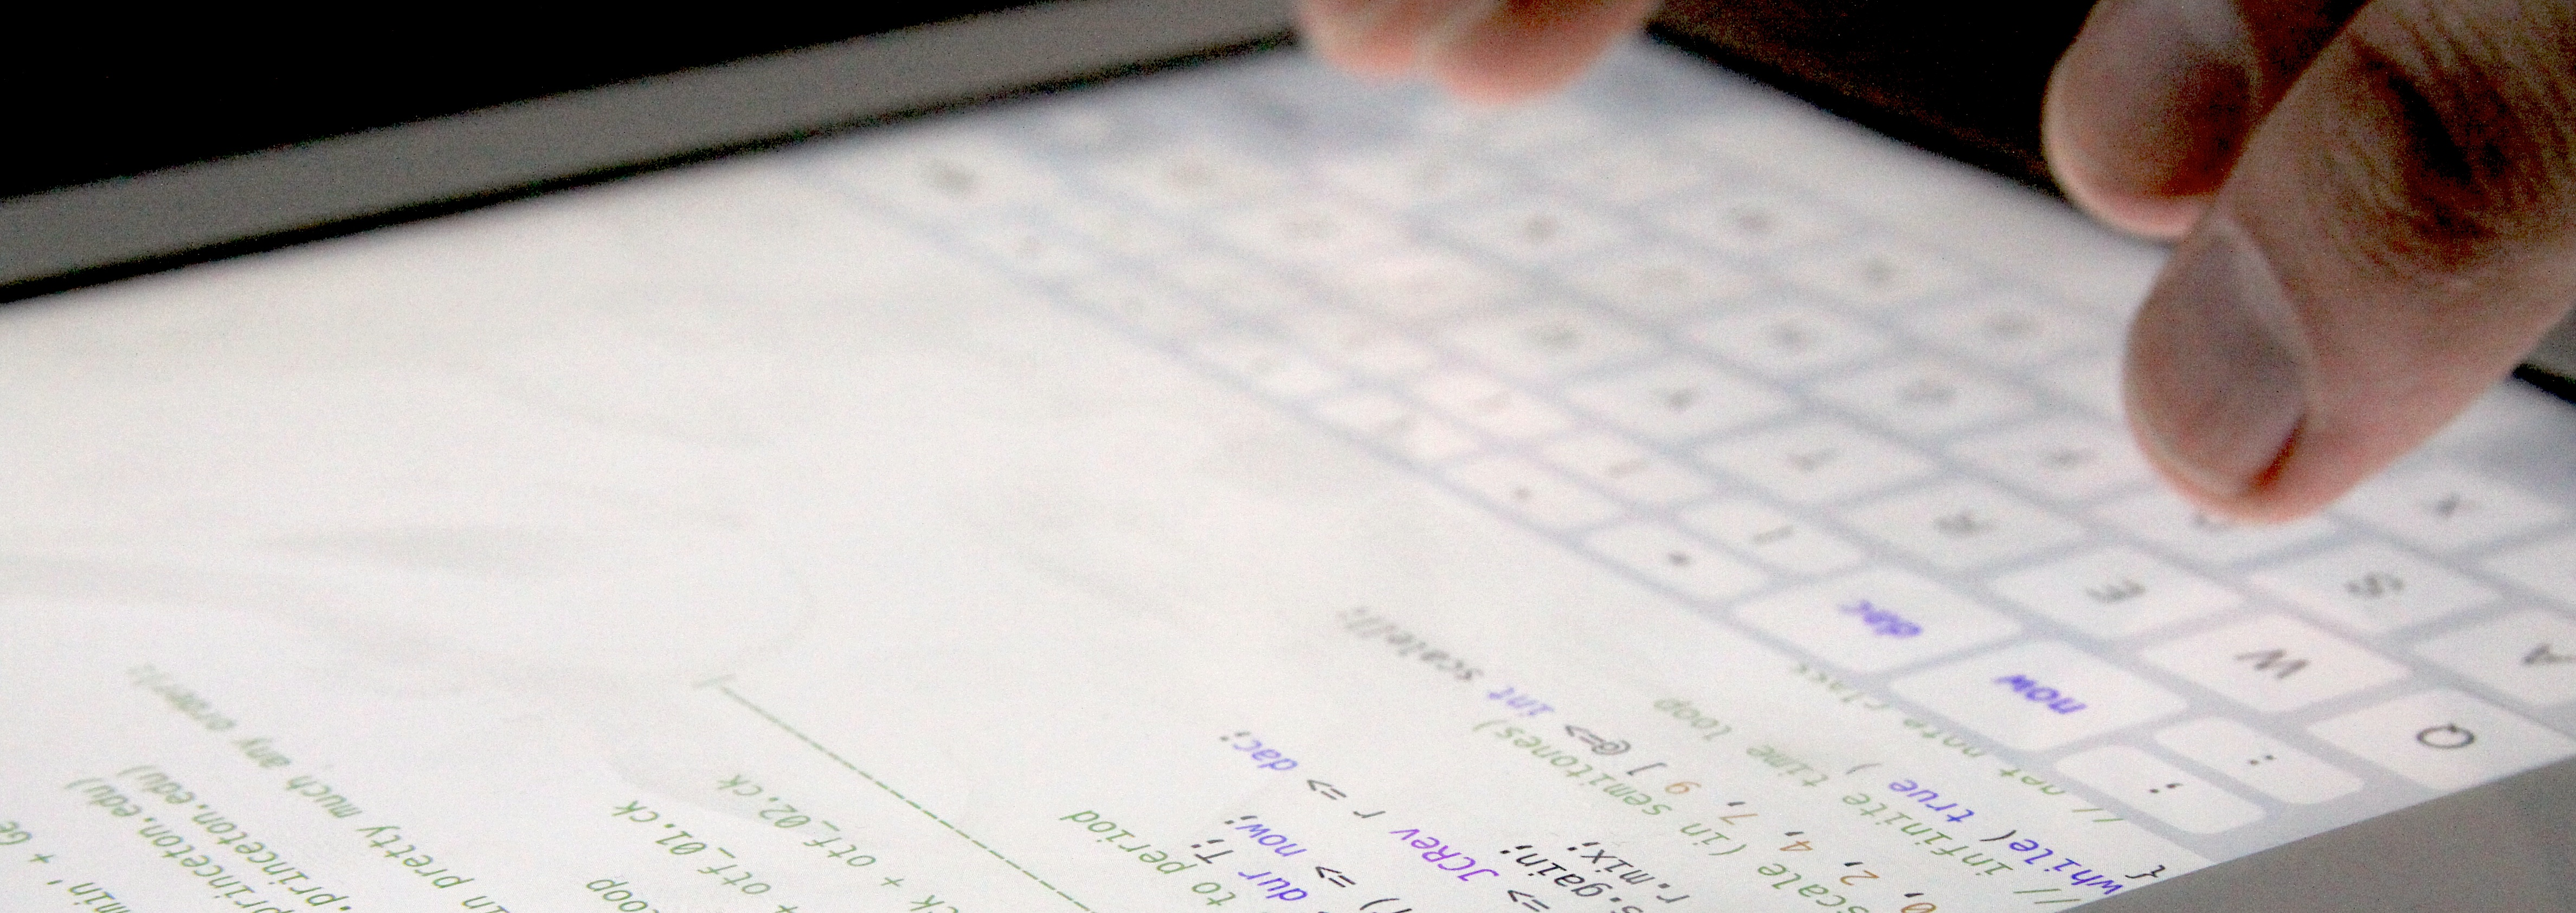
\includegraphics[width=1\textwidth]{figures/teaser.jpg}
	\caption{miniAudicle for iPad.}
	\label{fig:teaser}
}

% ***************************************** the document starts here ***************
\begin{document}
%
\capstartfalse
\maketitle
\capstarttrue
%
\begin{abstract}

We present a new software application for ChucK programming and performance on mobile touchscreen devices, miniAudicle for iPad. 
This application seeks to accommodate keyboard-based music software development as well as explore new music programming possibilities enabled by touch interfaces. 
To this end, it provides a textual code Editor mode optimized for touchscreen typing, a live-coding-oriented Player mode, and collaborative network performance via a Connect mode. 
The combination of these features provides a foundation for the exploration of musical programming on mobile touchscreen devices. 

\end{abstract}
%

\section{Introduction}\label{sec:introduction}

Recent years have seen dramatic shifts in mainstream human-computer interaction, as multitouch mobile phone and tablet devices have taken hold of the popular technological zeitgeist. 
These trends have caused massive changes in both the way we work with technology and the way we think about technology. 
The prevalence of touchscreens has given software designers and researchers a vast dimension of interaction models to work with, a dimension we have only begun to explore. 
The intrinsic mobility and effective ubiquity of these devices have further increased the depth and transparency of mainstream computing. 

In this work we examine an often overlooked possibility of mobile touchscreen computing, that of music software programming. 
To this end, we have designed and implemented an iPad application for real-time coding and performance in the ChucK music programming language~\cite{wang2008chuck}. 
This application shares much of its design philosophy, source code, and visual style with the miniAudicle editor for desktop ChucK development~\cite{salazar2006miniaudicle}, and thus we call it \textit{miniAudicle for iPad}. 

The goals miniAudicle for iPad are to provide a satisfactory method for creation and editing of non-trivial ChucK code, and to fully leverage the interaction possibilities of mobile touchscreen devices. 
Our approach to these goals is to provide three complementary modes: Editor mode, Player mode, and Connect mode. 
Editor mode aims to provide the best code editor possible given the limitations of typing text on a touchscreen. 
Player mode allows users to play and modify scripts concurrently using ChucK's intrinsic on-the-fly programming capabilities. 
It aims to enable multitouch live-coding and performance techniques that would be difficult or impossible on traditional desktop computers. 
Connect mode extends Player mode to a networked performance, in which multiple players on network connected iPads collaboratively live-code music in real-time. 
We believe the combination of these three systems makes miniAudicle for iPad a compelling mobile system for music programming and live coding. 

\section{Related Work}\label{sec:relatedWork}

Naturally, much of this work draws from desktop computer-based environments for music programming, such as the original desktop miniAudicle~\cite{salazar2006miniaudicle}, the Audicle~\cite{wang2004audicle}, and SuperCollider~\cite{mccartney2002supercollider}. 
Each of these systems combines conventional code development with performative interfaces, explicitly enabling live coding of music~\cite{collins2003live}. 
The CoAudicle extends musical live-coding to interactive network-enhanced performance between multiple performers~\cite{wang2005coaudicle}. 

More recent developments in live-coding software systems have lead to ixi lang, which complements SuperCollider with a domain-specific language designed for live-coding~\cite{magnusson2011ixi}, and Overtone, which uses the Clojure programming language to control SuperCollider's core synthesis engine~\cite{aaron2013overtone}. 
Ableton's Live software is not technically a programming system, but its model of sequencing distinct musical ``objects'' has influenced our development of miniAudicle for iPad's Player mode~\cite{ableton}. 

In the domain of general purpose computing, TouchDevelop is a touch-based text programming environment designed for use on mobile phones, in which programming constructs are selected from a context-aware list, diminishing the dependence on keyboard-based text input~\cite{Tillmann2011}. 
Codea is a Lua-based software development system for iPad in which text editing is supplemented with touch gestures for parameter editing and mapping~\cite{saens2014codea}. 
Many canonical interactions for music sequencing and programming on a touchscreen device can be traced back to the Reactable \cite{jorda2007reactable} and the work of Davidson and Han~\cite{davidson2006synthesis}, two early explorations of the application of touchscreen technology to computer music. 

A number of software applications from iPhone developer Smule have begun to delineate the space of possibilities for mobile music computing~\cite{wang2009smule}. 
Ocarina is both a musical instrument, designed uniquely around the iPhone's interaction capabilities, and a musical/social experience, in which performers tune in to each others' musical renditions around the world~\cite{wang2014ocarina}. 
World Stage takes this model a step further, by congregating groups of users into a live ``American Idol''-like panel for critiquing and rating performances on a mobile phone instrument~\cite{wang2011world}. 
The conceptual background of these endeavors stems from research in the Princeton Laptop Orchestra~\cite{smallwood2008plork}, the Stanford Laptop Orchestra~\cite{wang2009slork}, and the Small Musically Expressive Laptop Toolkit~\cite{fiebrink2007smelt}.
Each of these efforts examines the explicit affordances of the laptop as a musical instrument in its own right, rather than as a generic unit of computing. 

% addl references
%MadPad~\cite{kruge2011madpad}
%ShEMP~\cite{bortz2012shemp}

\section{Background and Motivations}\label{sec:backgroundAndMotivations}

In our experience, mobile touchscreen devices have been largely overlooked for use in computer music software development. 
As these technologies have become widespread, it is not sufficient to sit back and watch inappropriate, pre-existing interaction models be forced into the mobile touchscreen metaphor. 
Rather, it is incumbent upon the research community to explore how best to leverage the unique assets and drawbacks of this new paradigm, which is evidently here to stay. 
Similar trends might be seen in the shift in computer music from mainframes and dedicated synthesizers to the personal computer in the 1980s, and then to the laptop, now ubiquitous in modern computer music performance practice. 
As these computing paradigms gave way from one to another, the software tools and interaction metaphors adjusted to better take advantage of the dominant paradigm. 

Therefore, our overriding design philosophy for miniAudicle for iPad was not to transplant a desktop software development environment to a tablet, but to consider what interactions the tablet might best provide for us. 
At the same time, it is not entirely reasonable to completely discard the desktop metaphor, which, in our case, is that of typing code into an editor. 
Ultimately, the fundamental unit of ChucK programming is text. 

For these reasons we have firstly sought to create the best code editing interface we could for a touchscreen device. 
Typing extensive text documents on touchscreens is widely considered undesirable. 
However, using a variety of popular techniques like syntax highlighting, auto-completion, and extended keyboards, we can optimize this experience.
With these techniques, the number of keystrokes required to enter code is significantly reduced, as is the number of input errors produced in doing so. 
Additional interaction techniques can improve the text editing experience beyond what is available on the desktop. 
For example, one might tap a unit generator typename in the code window to bring up a list of alternative unit generators of the same category (e.g. oscillators, filters, reverbs). 
Tapping a numeric literal could bring up a slider to set the value, where a one-finger swipe adjusts the value and a two finger pinch changes the granularity of those adjustments. 

Secondly, we believe that live-coding performance is a fundamental aspect of computer music programming, and contend that the mobile touchscreen paradigm is uniquely equipped to support this style of computing. 
Live-coding often involves the control and processing of many scraps of code, with multiple programs interacting in multiple levels of intricacy. 
Direct manipulation, the quintessential feature of a multitouch screen, might allow large groups of "units" --- individual ChucK scripts --- to be efficiently and rapidly controlled in real-time. 
This is the basis of miniAudicle for iPad's \textit{Player} mode, in which a user assembles and interacts with any number of ChucK programs simultaneously. 

Furthermore, we fundamentally believe in the power of the network. 
As seen in Ocarina, World Stage, and related systems, musical interactions mediated by a wide-area computer network can create unique musical experiences among its users. 
These interactions are distinctive from those possible in the real world, being effectively anonymous and instantaneous, and having the potential to engage countless users on a massive scale. 
We have sought to apply these concepts to musical live-coding in \textit{Connect} mode, an extension to Player mode that enables collaborative musical programming over the network. 

Lastly, we are interested in the physicality of the tablet form-factor itself. 
The iPad's hardware design presents a number of interesting possibilities for musical programming. 
For instance, it is relatively easy to generate audio feedback by directing sound with one's hand from the iPad's speaker to its microphone. 
A ChucK program could easily tune this feedback to musical ends, while the user  maintains manual control over the presence and character of the feedback. 
The iPad contains a number of environmental sensors, including an accelerometer, gyroscope, and compass. 
ChucK programs that incorporate these inputs might use them to create a highly gestural musical interaction, using the tablet as both an audio processor and as a physical controller. 

\section{Interaction Design}\label{sec:interactionDesign}

Interaction in miniAudicle for iPad is divided between three primary modes, Editor mode, Player mode, and Connect mode, described individually below. 
Several interface elements are common to all three modes.
First of these is a script browser which allows creating, managing, and selecting individual ChucK programs to load into either mode. 
Views of ChucK's console output (such as error messages and internal diagnostics) and a list of the ChucK shreds (processes) running in the system are available from the main application toolbar. 
This toolbar also contains a switch to toggle between Editor and Player modes, while Connect mode, an enhancement of Player mode, is accessed from a button within that mode. 

\subsection{Editor}

Editor mode is the primary interface for writing and testing ChucK code. 
This mode is centered around a touch-based text editing view, in which a single ChucK source document is presented at a time (Figure \ref{fig:editor}). 
The document to edit can be changed via the script browser. 
Once a document is loaded, the text view provides a number of features common to programming text editors, such as syntax-based text coloring and integrated error reporting. 
Additionally, the on-screen keyboard has been supplemented with ChucK-specific keys for characters and combinations thereof that appear frequently in ChucK programs. 
These additional keys include the chuck operator (\texttt{=>}) and its variants, mathematical operators, a variety of brace characters, additional syntax characters, and the \texttt{now}/\texttt{dac} keywords. 

\begin{figure}[h]
	\centering
		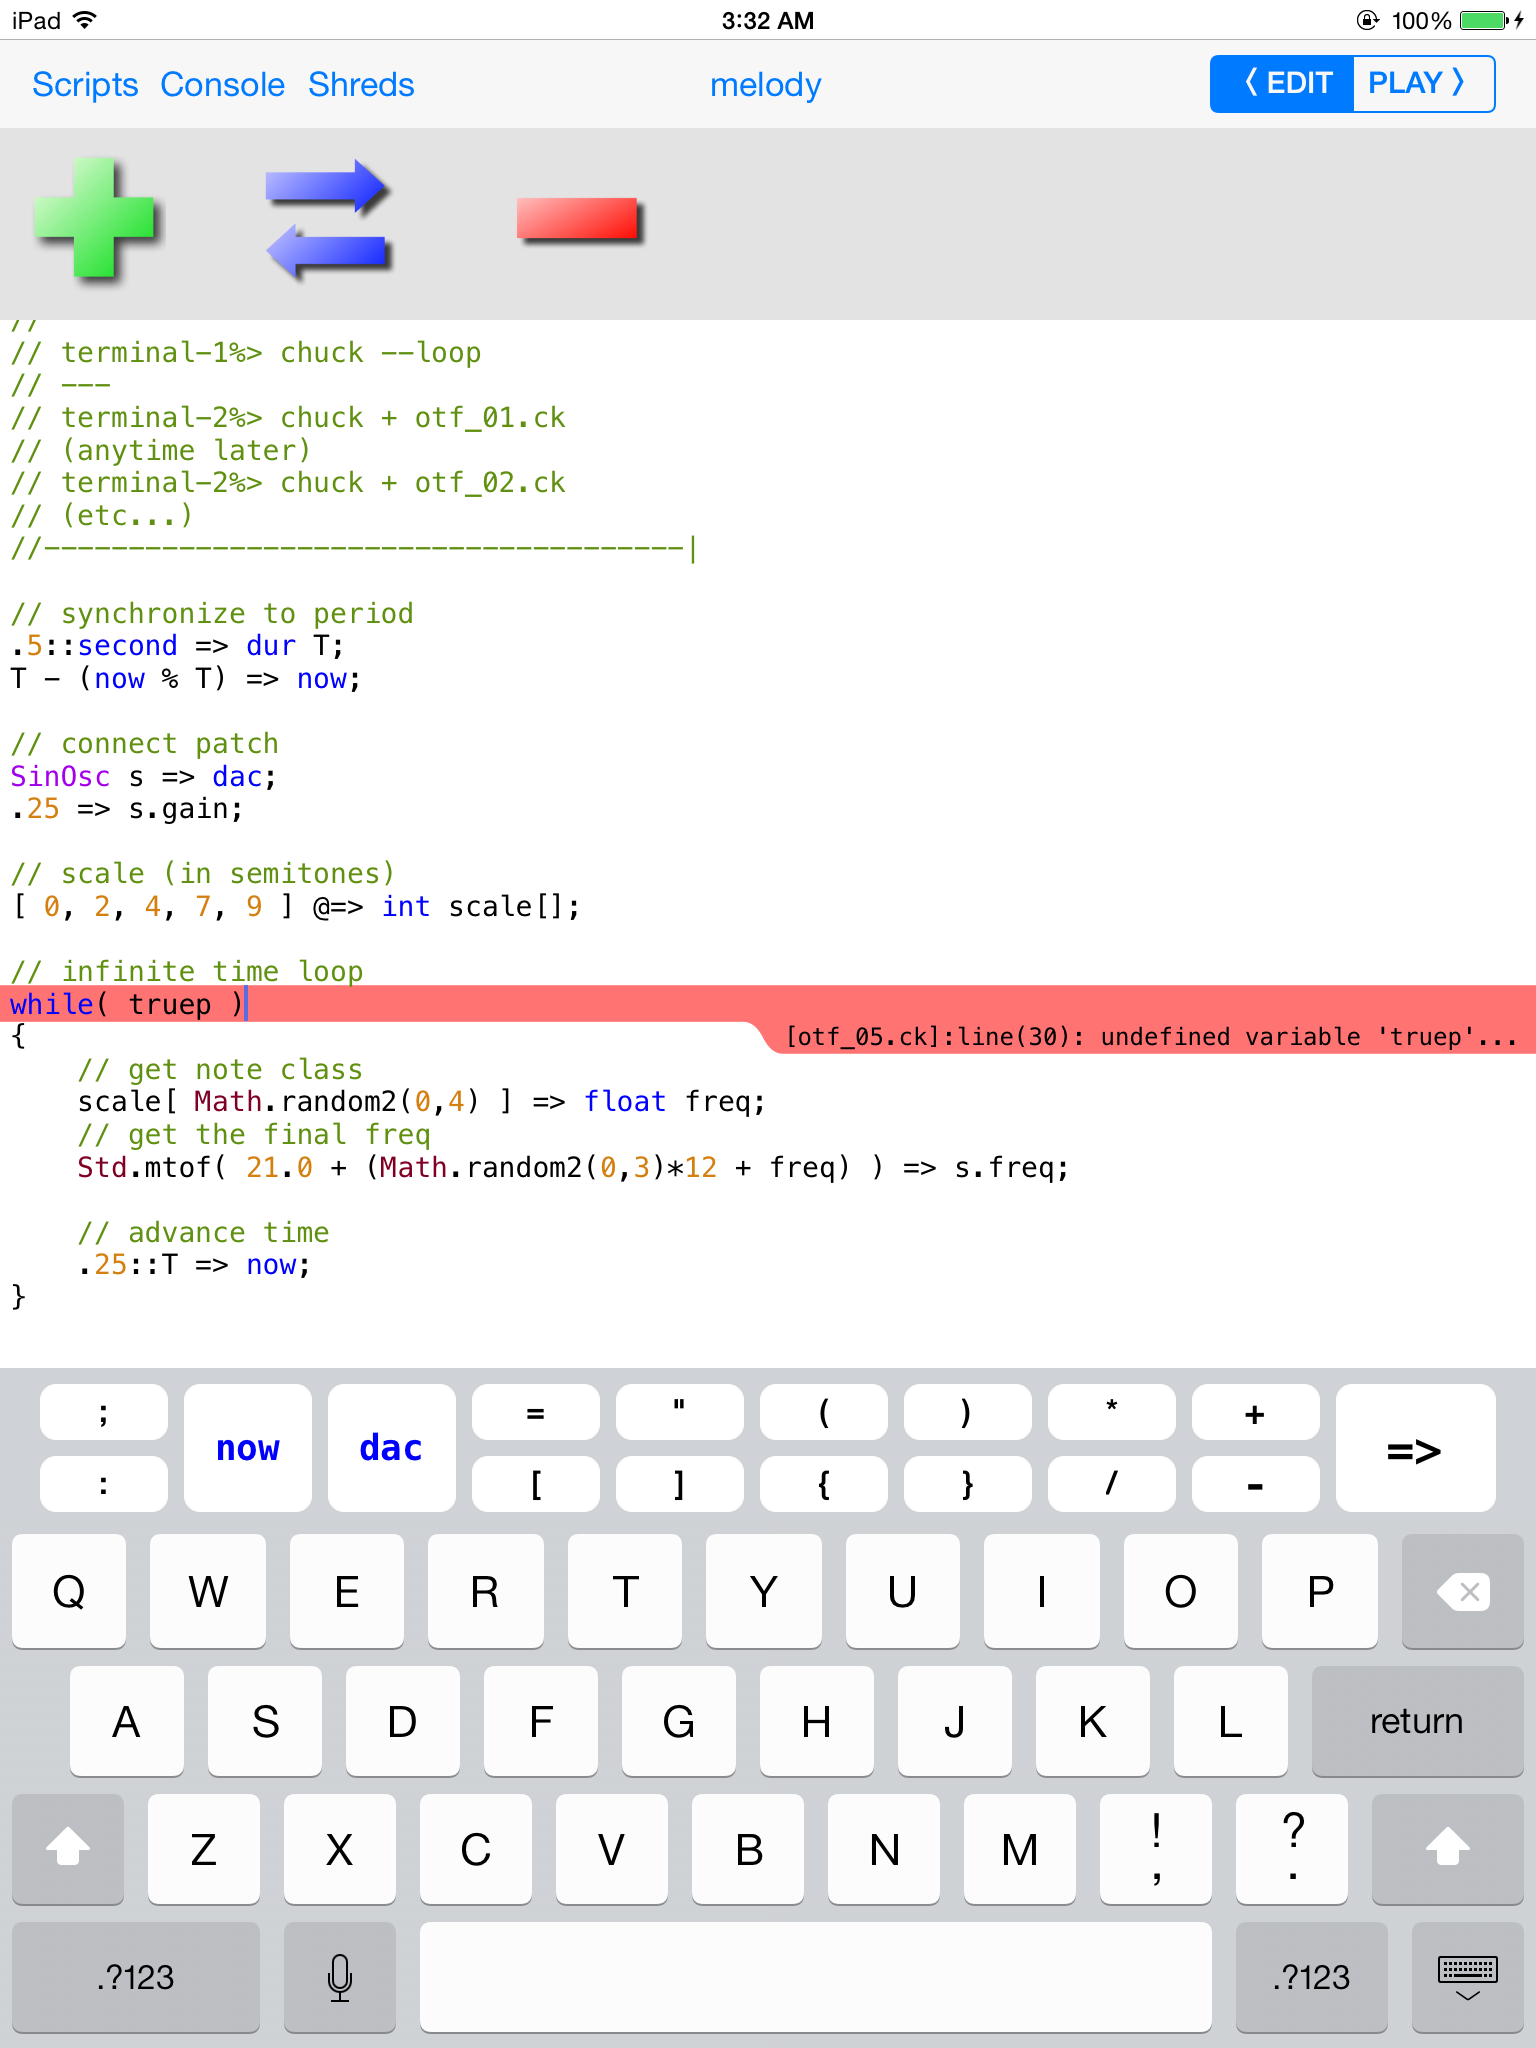
\includegraphics[width=0.45\textwidth]{editor.png}
	\caption{Editor mode. }
	\label{fig:editor}
\end{figure}

This mode also features buttons for adding, replacing, and removing the currently edited ChucK script, enabling a small degree of on-the-fly programming and performance capabilities. 

\subsection{Player}

Player mode is designed for live performance, on-the-fly programming, and real-time musical experimentation . 
In this mode, selected ChucK scripts are displayed as small tabs in a large open area (Figure \ref{fig:player}). 

\begin{figure}[h]
	\centering
		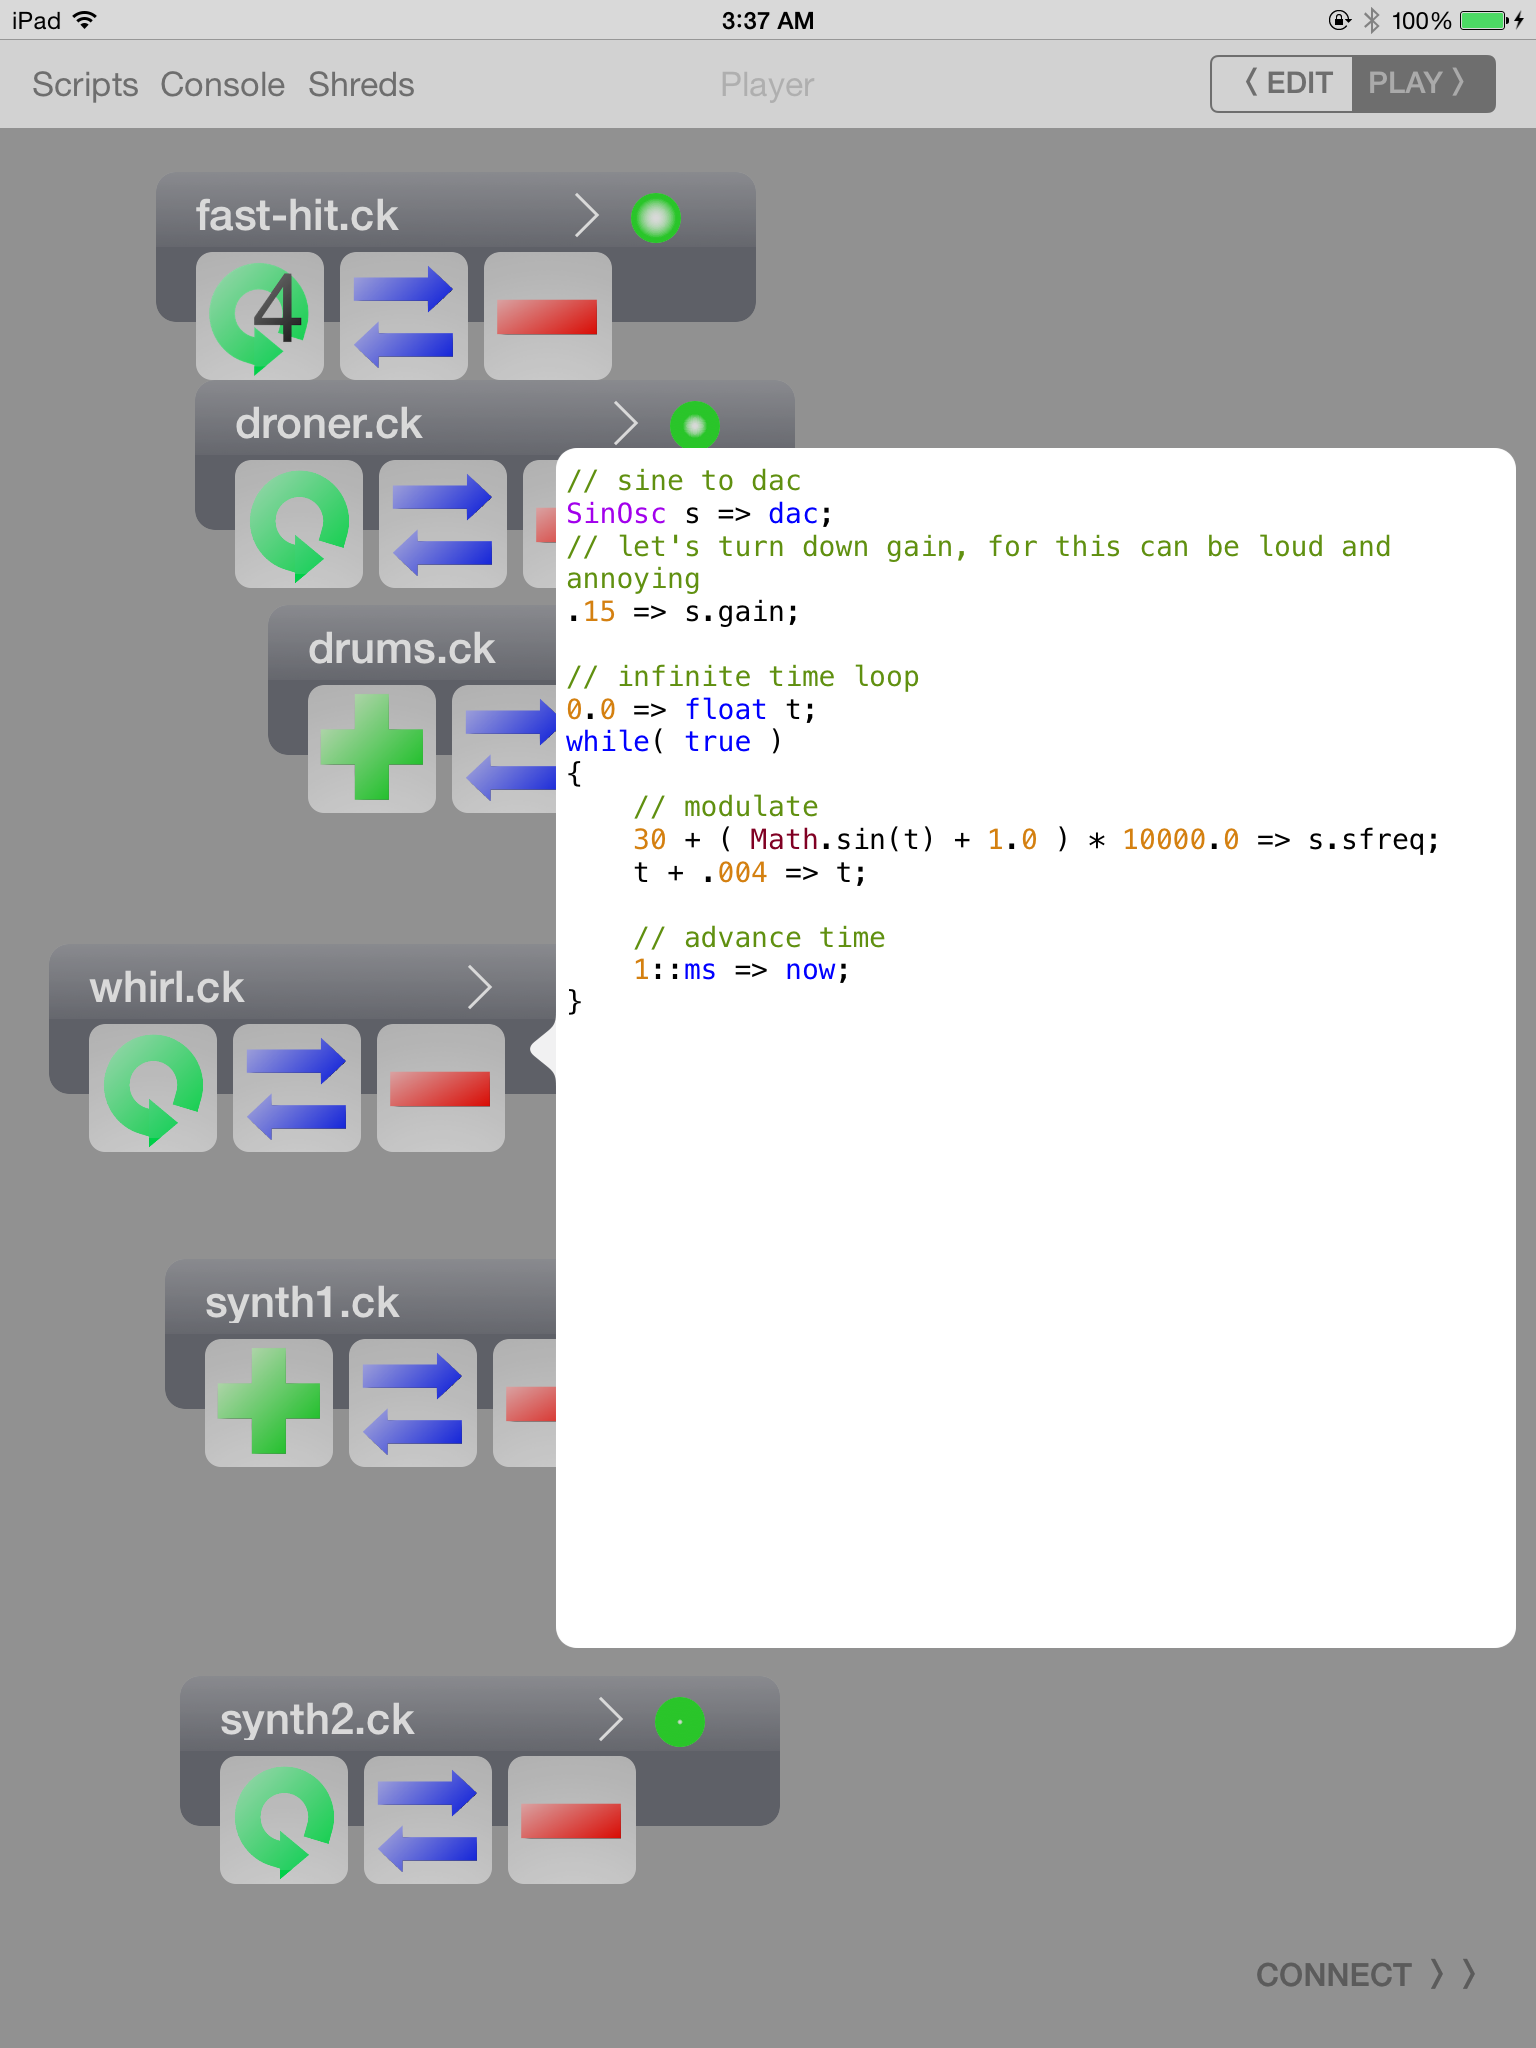
\includegraphics[width=0.45\textwidth]{figures/player.png}
	\caption{Player mode. }
	\label{fig:player}
\end{figure}

The script tabs can be rearranged in the space by moving them with touch, with new tabs  created via the script browser. 
Each tab has prominent buttons to add the script the virtual machine, replace it, and remove it, enabling basic on-the-fly programming of each script in the player (Figure \ref{fig:tab}).\footnote{
A brief ChucK on-the-fly programming primer: adding a script causes it to be compiled and executed, generating whatever sounds and manipulating whatever data it was programmed to do. 
A script running in the virtual machine is referred to as a \textit{shred}. 
Replacing it causes the currently executing version of the shred to be removed, and the latest version of the script to replace it. 
Removing it simply stops it from executing.}
A script can be added multiple times, and currently running scripts are visualized by one or more glowing dots on that scripts tab. 
Pressing a dot removes the iteration of the script that that dot represents. 
An arrow button on the tab pops open a mini-editor for that script, from which the full editor mode can also be opened if desired. 

Pressing and holding the add button will cause three more buttons to appear below it, on the left, and on the right: one causes the program to loop infinitely (until it is manually removed), one loops it a user-selected number of times, and one allows sequencing a different script after this script completes. 
Finite looping and sequencing can be used in conjunction with one another, allowing scripts to run a number of times before advancing to the next script in the sequence. 
Pressing and holding any tab outside of the button areas will cause delete buttons to appear above all tabs, a common interaction for deleting items from collections in touchscreen apps. 

The design of Player mode is theoretically not limited to the touchscreen environment; one can easily imagine a similar design for desktop computers using mouse-and-keyboard interaction. 
However, touchscreens allow a level of direct, simultaneous interaction with Player mode that is not feasible using keyboard-and-mouse. 
Using touch control, multiple scripts can be fired off or removed instantly, different combinations of shreds can be quickly configured and evaluated, and multiple edited scripts can be replaced on-the-fly in tandem. 
These sorts of interactions are not impossible in mouse-and-keyboard environments, but typically are held back by the sluggishness of mouse navigation, or require the use of arcane key command sequences. 

\begin{figure}[h]
	\centering
		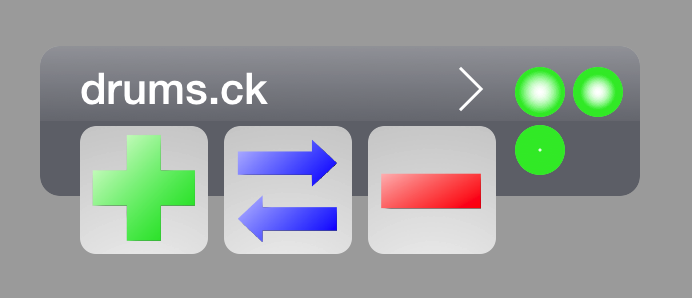
\includegraphics[width=0.45\textwidth]{figures/tab.png}
	\caption{An individual tab in player mode. 
	In addition to buttons for on-the-fly programming, the green dots represent individual program instances (shreds) that are currently running. 
	Pressing a green dot removes that instance. 
	Pressing the disclosure arrow opens a mini-editor for the script, and modified versions of the script can replace a running shred. 
	}
	\label{fig:tab}
\end{figure}

\subsection{Connect}

Connect mode, an extension of Player mode, allows miniAudicle programmers to collaboratively perform and hack ChucK code over the network (Figure \ref{fig:connect}). 
In this mode, multiple Player sessions from disparate iPads are essentially combined into a single session. 
As networked players add, remove, and modify programs, these changes are propagated to each other player in the session, constructing a single, collaborative performance. 
Furthermore, looping and sequencing features of Player mode are also enabled in Connect mode, allowing for advanced musical twists and segues. 

Connect mode is initiated by pressing the ``Connect'' button in Player mode, opening a small dialog to allow setting connection parameters, such as username, geographic location, and whether to join an existing session or to create a new one. 
Once a user is connected to a session (possibly one that he or she just created), a list of other users in the session (if any) is displayed. 
Each ChucK script tab displays the username of the player who originated it. 
Tabs are also color-coded to indicate which are owned by the local player and which are owned by remote players --- a player can only interact with scripts he or she created, although the source code for each script can be examined by anyone in the session. 
We intend for the ability to view another player's code to spur code sharing and the dissemination of music software techniques. 
Finally, a player may disconnect from the session at any time by pressing a ``Disconnect'' button. 

\begin{figure}[hb]
	\centering
		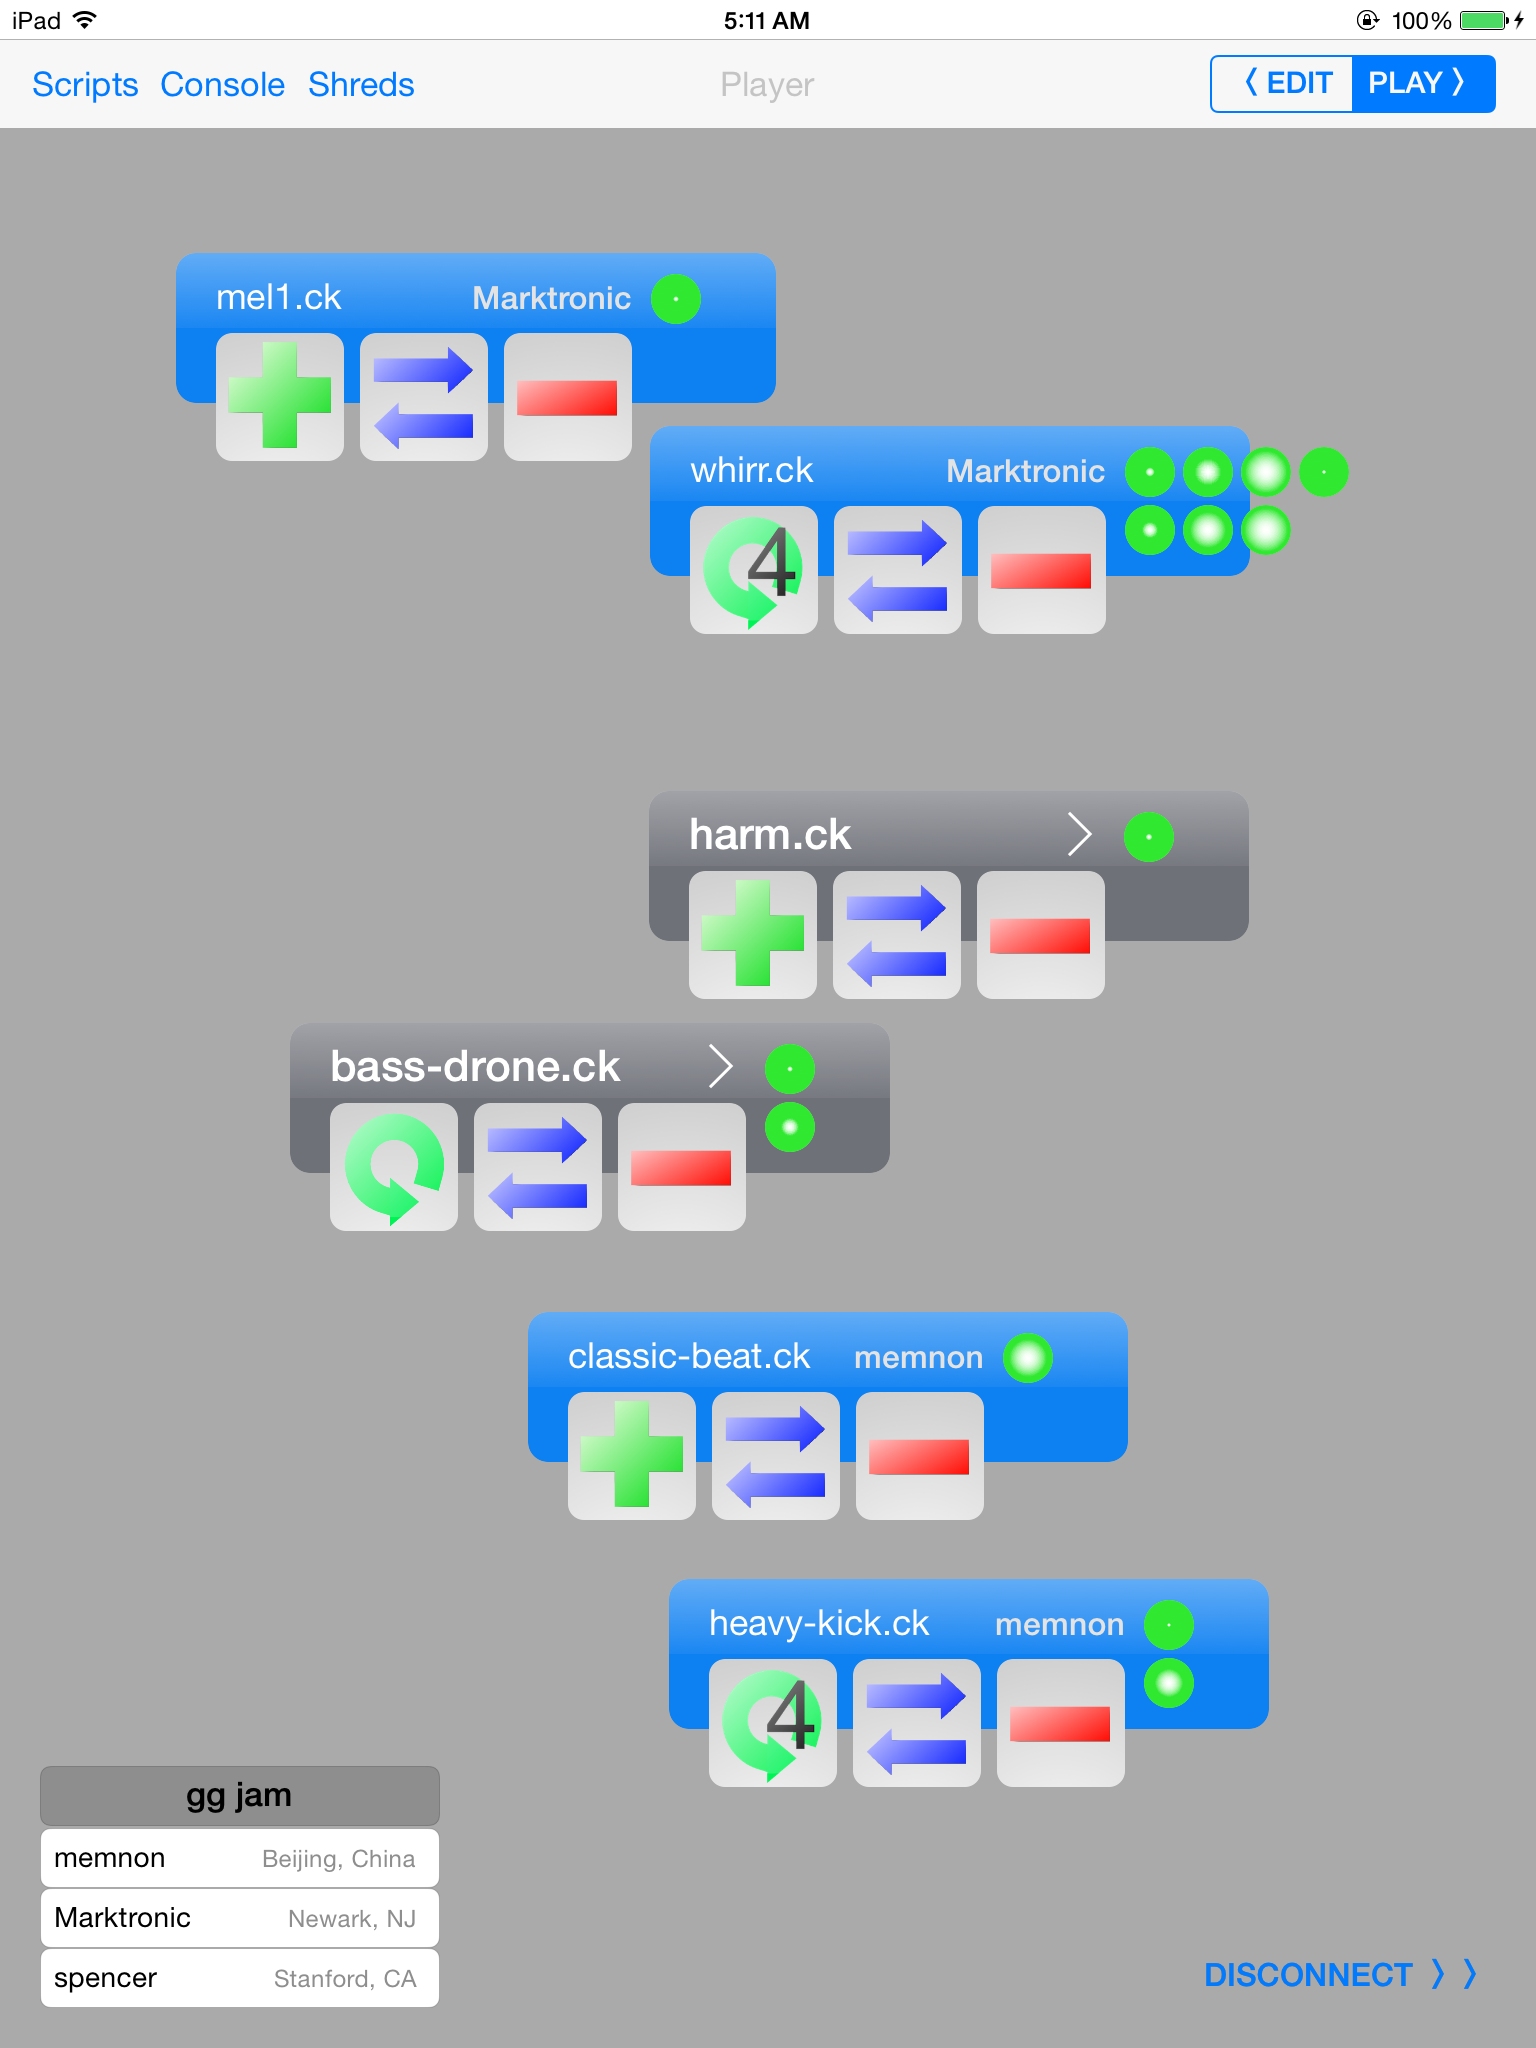
\includegraphics[width=0.45\textwidth]{figures/connect.png}
	\caption{Connect mode. }
	\label{fig:connect}
\end{figure}

\subsubsection{Network Back-end}

The network interactions that encompass Connect mode are supported by a central miniAudicle server, which manages players, sessions, and the interactions between them. 
The server software is implemented in Python using the Twisted framework,\footnote{https://twistedmatrix.com/} and uses Representational State Transfer (REST) over HTTP to communicate with the client. 
Each action a player takes in Connect mode is encoded as a JSON data structure, and uploaded to the server. 

While engaged in a Connect session, the client software continuously polls the server for new actions, such as a user adding a shred or modifying and replacing an existing shred. 
When a new action is received from the server, it is immediately enacted on the client. 
In effect, each client of the session simultaneously runs every ChucK program from every user in the session. 
As a result, sample-accuracy between every shred is maintained in a given session on a given client. 
Using ChucK's innate strong-timing functionality, intricate and consistent rhythmic patterns can be constructed between programs from multiple individuals in a session. 
However, latency must obviously exist between when, for example, one user adds a shred on his own tablet, and when that action is reflected on another player's tablet over the network. 
As the practice of networked live-coding in ChucK matures, we anticipate the development of software techniques to address the drawbacks of these physical realities. 

\section{Future Work and Conclusions}\label{sec:conclusions}

Of critical importance in any interactive software system is the evaluation of that system with respect to its goals and overall user experience. 
We intend to assess miniAudicle for iPad in these regards in upcoming research efforts. This might involve formalized user testing, with users spanning a range of skill levels in ChucK programming, statistical analysis of Connect-mode performance sessions, and the development of touchscreen-based live coding performances in the concert setting. 

Yet to be explored in this system is the deeper social dynamics of a networked live-coding community, and how the design of the Connect system might provoke or discourage certain musical behaviors. 
For example, networked live-coding sessions could be opened for anyone to listen in, and especially popular or productive players on the miniAudicle network might be promoted within it. 
We chose not to enable explicit communication between Connect players other than the ChucK code itself; it merits consideration whether allowing in-session chat would lead to stronger musical collaboration, or if it would distract from purely musical creative processes.  
The experience of developing and supervising the World Stage~\cite{wang2011world} provides many lessons for such building of online musical communities. 

We believe that miniAudicle for iPad provides a compelling foundation for the exploration of music programming and live-coding performance on mobile touchscreen devices. 
A touch-augmented text editor, advanced live-coding functionality, and networked performance features combine into a computer music environment that leverages the principal features of touchscreen computing while retaining the immense expressivity of textual programming. 
As we apply final touches and polish, we will release miniAudicle for iPad both in the Apple App Store and as source code under an open source license. 
We hope that this work might help to compel further consideration and research of music programming on mobile touchscreen systems. 


%%%%%%%%%%%%%%%%%%%%%%%%%%%%%%%%%%%%%%%%%%%%%%%%%%%%%%%%%%%%%%%%%%%%%%%%%%%%%
%bibliography here
\bibliography{omni.bib}

\end{document}
